\documentclass[oneside]{article}

%%%%%%%%%%%%%%%%%%%%%%%%%%%%%%%%%%%%%%%%%%%%%%%%%%%%%%%%%%%%%%%%%%%%%%%%
% For Greek Chars using pdfLaTeX                                       %
%%%%%%%%%%%%%%%%%%%%%%%%%%%%%%%%%%%%%%%%%%%%%%%%%%%%%%%%%%%%%%%%%%%%%%%%

\usepackage[english, greek]{babel}
\usepackage{fontspec}

%%%%%%%%%%%%%%%%%%%%%%%%%%%%%%%%%%%%%%%%%%%%%%%%%%%%%%%%%%%%%%%%%%%%%%%%
% Other useful packages                                                %
%%%%%%%%%%%%%%%%%%%%%%%%%%%%%%%%%%%%%%%%%%%%%%%%%%%%%%%%%%%%%%%%%%%%%%%%

\usepackage[x11names]{xcolor}
\usepackage[pdfusetitle]{hyperref}
\usepackage[most]{tcolorbox}
\usepackage[bf]{caption} 
\usepackage[automark]{scrlayer-scrpage}
\usepackage[newfloat]{minted}
\usepackage{amssymb, bm, amsmath}
\usepackage{enumerate}
\usepackage{multicol}
\usepackage{float}
\usepackage{array,tabularx}
\usepackage{fontawesome5}
\usepackage{colortbl}
\usepackage{dirtree}
\usepackage{menukeys}
\usepackage{mathtools}
\usepackage{listings}
\usepackage{amsthm}
\usepackage{mdframed}
\usepackage{accsupp}
\usepackage{multirow}
\usepackage{breqn}
\usepackage{cancel}
\usepackage{layouts}

%%%%%%%%%%%%%%%%%%%%%%%%%%%%%%%%%%%%%%%%%%%%%%%%%%%%%%%%%%%%%%%%%%%%%%%%
% Shortcut creation                                                    %
%%%%%%%%%%%%%%%%%%%%%%%%%%%%%%%%%%%%%%%%%%%%%%%%%%%%%%%%%%%%%%%%%%%%%%%%

\let\b\textbf
\let\t\texttt
\let\u\underline

%%%%%%%%%%%%%%%%%%%%%%%%%%%%%%%%%%%%%%%%%%%%%%%%%%%%%%%%%%%%%%%%%%%%%%%%
% Font Setup                                                           %
%%%%%%%%%%%%%%%%%%%%%%%%%%%%%%%%%%%%%%%%%%%%%%%%%%%%%%%%%%%%%%%%%%%%%%%%

\setmainfont{Open Sans}
\setmonofont{Droid Sans Mono}

%%%%%%%%%%%%%%%%%%%%%%%%%%%%%%%%%%%%%%%%%%%%%%%%%%%%%%%%%%%%%%%%%%%%%%%%
% Pagestyle options                                                    %
%%%%%%%%%%%%%%%%%%%%%%%%%%%%%%%%%%%%%%%%%%%%%%%%%%%%%%%%%%%%%%%%%%%%%%%%

\clearpairofpagestyles 
\newlength{\headerrulelength}
\setlength{\headerrulelength}{3ex}

\newcommand*{\headerrule}{
    \rule[-1ex]{0.1em}{\headerrulelength}
}

% Define headers:
\lehead{% Left, even head
    \llap{
        \pagemark\enskip\headerrule
    }
    \enskip\headmark
}

\rohead{% Right, odd head
    \headmark\enskip
    \rlap{
        \headerrule\enskip\pagemark
    }
}

%%%%%%%%%%%%%%%%%%%%%%%%%%%%%%%%%%%%%%%%%%%%%%%%%%%%%%%%%%%%%%%%%%%%%%%%
% Color definition                                                     %
%%%%%%%%%%%%%%%%%%%%%%%%%%%%%%%%%%%%%%%%%%%%%%%%%%%%%%%%%%%%%%%%%%%%%%%%

\colorlet{g1}{black!70}
\colorlet{g3}{black!40}
\colorlet{g6}{black!05}
\definecolor{darklink}{RGB}{48, 62, 116}
\definecolor{darklinkGreen}{RGB}{65, 107, 60}

%%%%%%%%%%%%%%%%%%%%%%%%%%%%%%%%%%%%%%%%%%%%%%%%%%%%%%%%%%%%%%%%%%%%%%%%
% Caption options                                                      %
%%%%%%%%%%%%%%%%%%%%%%%%%%%%%%%%%%%%%%%%%%%%%%%%%%%%%%%%%%%%%%%%%%%%%%%%

\addto\captionsenglish{\renewcommand{\figurename}{Σχήμα}}
\addto\captionsenglish{\renewcommand{\tablename}{Πίνακας}}
\addto\captionsenglish{\renewcommand{\bibname}{Πηγές}}
\addto\captionsenglish{\renewcommand{\lstlistingname}{Κώδικας}}
\addto\captionsenglish{\renewcommand{\listingname}{Κώδικας}}
\addto\captionsenglish{\renewcommand{\chaptername}{Κεφάλαιο}}
\addto\captionsenglish{\renewcommand{\contentsname}{Περιεχόμενα}}

%%%%%%%%%%%%%%%%%%%%%%%%%%%%%%%%%%%%%%%%%%%%%%%%%%%%%%%%%%%%%%%%%%%%%%%%
% Hyperref options                                                     %
%%%%%%%%%%%%%%%%%%%%%%%%%%%%%%%%%%%%%%%%%%%%%%%%%%%%%%%%%%%%%%%%%%%%%%%%

\hypersetup{
    colorlinks=true,
    allcolors=darklink,
    urlcolor=darklinkGreen,
    plainpages=false,
    pdftitle={Συμμετρική Κρυπτογραφία},
    pdfsubject={Συμμετρική Κρυπτογραφία},
    pdfcreator={LaTeX with hyperref},
    pdfauthor={Αλέξανδρος Κόρκος},
    bookmarksnumbered=true,
    pdfdisplaydoctitle,
    pdfkeywords={%
        cryptography,%
        symmetric,%
        rc4,%
        otp,%
        shift-cipher,%
        vigenere-cipher,%
        perfect-secrecy,%
        aes,
        avalanche-effect 
    }
}

\newcommand{\Rule}{\rule{\linewidth}{0.5mm}}

%%%%%%%%%%%%%%%%%%%%%%%%%%%%%%%%%%%%%%%%%%%%%%%%%%%%%%%%%%%%%%%%%%%%%%%%
% Options                                                              %
%%%%%%%%%%%%%%%%%%%%%%%%%%%%%%%%%%%%%%%%%%%%%%%%%%%%%%%%%%%%%%%%%%%%%%%%


\newtheorem*{definition}{Ορισμός}

\newcommand{\Mod}[1]{\ (\mathrm{mod}\ #1)}

\setcounter{MaxMatrixCols}{16}

%%%%%%%%%%%%%%%%%%%%%%%%%%%%%%%%%%%%%%%%%%%%%%%%%%%%%%%%%%%%%%%%%%%%%%%%
% Document begin                                                       %
%%%%%%%%%%%%%%%%%%%%%%%%%%%%%%%%%%%%%%%%%%%%%%%%%%%%%%%%%%%%%%%%%%%%%%%%

\begin{document}
    
\begin{titlepage}

    \begin{figure}[!htb]
        \centering
        \begin{minipage}{0.45\textwidth}
            \centering
            
\includegraphics[width=0.4\textwidth]{Images/logo_csd.png} % first figure itself
        \end{minipage}\hfill
        \begin{minipage}{0.45\textwidth}
            \centering
            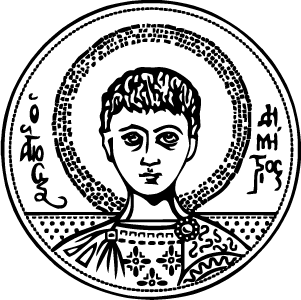
\includegraphics[width=0.5\textwidth]{Images/logo_auth.png} % second figure itself
        \end{minipage}
    \end{figure}
     
    \begin{center}
        \LARGE{Αριστοτέλειο Πανεπιστήμιο Θεσσαλονίκης}
        \vspace{5mm}
        \\ \Large{Τμήμα Πληροφορικής}
    \end{center}
    
    \vspace*{\fill}
    
    \begin{center}
        \Rule \\[0.4cm]
        { \LARGE 
            \textbf{Τεχνική αναφορά για NGE-06-03}\\[0.4cm]
            \emph{Συμμετρική Κρυπτογραφία}\\[0.4cm]
        }
        \Rule \\[0.4cm]
    \end{center}
    
    \vspace*{\fill}
    
    \begin{center}
        Αλέξανδρος Κόρκος \\
        \textbf{\href{mailto:alexkork@csd.auth.gr}{alexkork@csd.auth.gr}}\\
        \textbf{3870}
        \Rule \\[0.4cm]
        Θεσσαλονίκη, \today
    \end{center}
    
\end{titlepage}

\vspace*{\fill}

\begin{center}
    \href{https://creativecommons.org/licenses/by-nc-sa/4.0/deed.el}{
\includegraphics[scale=0.2]{Images/cc.png}} \\
    \Rule \\[0.4cm]
    Το έργο αυτό διατίθεται υπό τους όρους της άδειας \textbf{\href{https://creativecommons.org/licenses/by-nc-sa/4.0/deed.el}{Create Commons "Αναφορά Δημιουργού - Μη Εμπορική Χρήση - Παρόμοια Διανομή 4.0 Διεθνές"}}. \\ 
\end{center}

\newpage

\tableofcontents

\newpage

\section{Σύστημα μετατόπισης}

\subsection{Εκφώνηση} 

Το επόμενο κρυπτόγραμμα έχει ληφθεί:

\begin{center}
    \t{οκηθμφδζθγοθχυκχσφθμφμχγ}
\end{center}
Ο αλγόριθμος κρυπτογράφησης είναι ο εξής: 

Κάθε γράμμα του αρχικού μας μηνύματος αντικαθίσταται από την αριθμητική του τιμή (α: 1, ..., ω: 24). Ας είναι $x_0$ μία ρίζα του τριωνύμου $g(x) = x^2 + 3x + 1$. Σε κάθε αριθμό του μηνύματός μου προσθέτω την τιμή του πολυωνύμου $f(x) = x^5 + 3x^4 + 3x^3 + 7x^2 + 5x + 4$, στο $x_0$. Αντικαθιστώ κάθε αριθμό με το αντίστοιχο γράμμα. Βρείτε το αρχικό μήνυμα.

\subsection{Λύση}

\subsubsection{Μαθηματική επίλυση}

Από την εκφώνηση, γνωρίζω ότι $g(x_0) = 0$. 

Επίσης, θα απλοποιήσω την $f(x)$ μέσω της διαίρεση πολυωνυμικών συναρτήσεων έτσι ώστε να εκμεταλλευτώ την παραπάνω πληροφορία. Συνεπώς: 

\begin{equation} \label{eq:121}
    f(x) = g(x) \cdot h(x) \Rightarrow h(x) = \frac{f(x)}{g(x)} \Rightarrow h(x) = x^3+2x+1+\frac{3}{x^2+3x+1}
\end{equation}

Κάνοντας εφαρμογή της επιμεριστικής ιδιότητας στην (\ref{eq:121}), προκύπτει: 

\begin{equation} \label{eq:122}
    f(x) = (x^3+2x+1)\cdot g(x) + \frac{3}{\cancel{x^2+3x+1}}\cdot \cancel{g(x)} \Rightarrow f(x) = (x^3+2x+1) \cdot g(x) + 3
\end{equation}

Εξετάζω την συνάρτηση (\ref{eq:122}) για $x = x_0$:

\begin{equation} \label{eq:123}
    f(x_0) = (x_{0}^3+2x_0+1) \cdot \cancelto{0}{g(x_0)} + 3 \Rightarrow f(x_0) = 3
\end{equation}

Άρα, όλα τα γράμματα της αλφάβητα έχουν μετατοπιστεί κατά 3 θέσεις.

\subsubsection{Λεπτομέρειες για την υλοποίηση}

Εκτέλεση αρχείου:

\begin{center}
    \t{python shift.py}
\end{center}

Μια απλή υλοποίηση του συστήματος μετατόπισης, δηλαδή της συνάρτησης:

\begin{equation}
    D_n(x) = x - n \Mod{24}, n = 3
\end{equation}

\subsubsection{Συμπέρασμα}

Εκτελώντας το αρχείο για το μηνύματος εκφώνησης επιστρέφεται το εξής αποκρυπτογραφημένο μήνυμα:

\begin{center}
    \t{Μηδεις αγεωμετρητος εισιτω}
\end{center}

όπου ήταν φράση που βρισκόταν στην είσοδο της ακαδημίας του Πλάτωνα \footnote{\href{https://math.uoi.gr/images/pdf/mathclub/Leshi_12042016.pdf}{Πηγή}}.

\section{Το σύστημα του Vigenere}

\subsection{Εκφώνηση} 

Αποκρυπτογραφήστε το \href{https://github.com/drazioti/book_crypto/blob/master/symmetric_crypto/vigenere}{κείμενο [2]}, που κρυπτογραφήϑηκε με τον αλγόριϑμο του Vigenere.

Υποδ. Για την αποκρυπτογράφηση συστήνουμε να χρησιμοποιήσετε python. Για το μήκος του κλειδιού μπορείτε να χρησιμοποιήσετε έιτε test Kasiski ή την μέϑοδο του Friedman.

\subsection{Λύση} 

\subsubsection{Λεπτομέρειες για την υλοποίηση}

\paragraph{Βιβλιοθήκες}

\begin{itemize}
    \item functools
    \item re
\end{itemize}

\begin{center}
    \t{python vegenere.py <όνομα_αρχείου>}
\end{center}

Ως όνομα αρχείου δίνεται το αρχείο που θέλουμε να αποκρυπτογραφήσουμε.

Αρχικά, η βασικότερη συνάρτηση είναι η \t{kasiski}, που υλοποιεί την μέθοδο, σύμφωνα με \footnote{\href{https://pages.mtu.edu/~shene/NSF-4/Tutorial/VIG/Vig-Kasiski.html}{Μέθοδος Kasiski}}. Για να επιτευχθεί η frequency analysis, υλοποιείται η συνάρτηση \t{frequencyAnalysis} που βασίζεται στo άρθρο \cite{fa}.

\subsubsection{Συμπέρασμα}

Για να βρεθεί το αποκρυπτογραφημένο μήνυμα, διακρίνεται σε 3 βήματα που περιγράφονται στην συνέχεια.

Εκτελώντας λοιπόν το τεστ Kasiski, βρίσκετε πως το μήκος του κλειδιού είναι 7 χαρακτήρες. Για να φτάσουμε σε αυτό τον αριθμό, δοκιμάσθηκε η ομαδοποίηση του κειμένου με διαφορά πλήθη χαρακτήρων. Για ομαδοποίηση $\ge 5$ χαρακτήρων καταλήγουμε στο μήκος κλειδιού $= 7$. Για $< 5$ καταλήγουμε σε κλειδιά μήκους είτε 1 είτε 2 χαρακτήρων, που δεν αποκρυπτογραφούν το μήνυμα.

Στην συνέχεια, γίνετε ανάλυση συχνότητας γλώσσας (frequency analysis) για μήκος κλειδιού $= 7$. Η λέξη κλειδί στην οποία καταλήγουμε είναι \t{SHANNON}.

Τέλος, κάνοντας αποκρυπτογράφηση με λέξη κλειδί \t{SHANNON} προκύπτει το παρακάτω απόσπασμα μηνύματος (σχήμα \ref{fig:og_msg}) και συμπεραίνετε πως το κλειδί είναι ορθό μιας και το αποκρυπτογραφημένο μήνυμα απαρτίζεται από αγγλικές λέξεις.

\begin{figure}[H]
    \centering
    \t{A VERY SMALL PERCENTAGE OF THE POPULATION PRODUCES THE GREATEST PROPORTION OF THE IMPORTANT IDEAS THIS IS A KIN TO AN IDEA PRESENTED BY AN ENGLISH MATHEMATICIAN TURING THAT THE HUMAN BRAIN IS SOMETHING LIKE A PIECE OF URANIUM THE HUMAN BRAIN IF IT IS BELOW THE CRITICAL LAP AND YOU SHOOT ONE ...}
    \caption{Απόσπασμα του αποκρυπτογραφημένου μηνύματος}
    \label{fig:og_msg}
\end{figure}

\section{Κυκλική κύλιση}

\subsection{Εκφώνηση} 

Έστω ένα μήνυμα $m$, 16-bits. Θεωρούμε την κυκλική κύλιση προς τα αριστερά $ \ll \alpha$ κατά α bits. Έστω ότι $m$ κωδικοποιείται στο $c$ σύμφωνα με τον τύπο,

\begin{equation}
    c = m \oplus (m\ll6) \oplus (m\ll10)
\end{equation}

Βρείτε τον τύπο αποκωδικοποίησης. Δηλαδή, γράψτε το $m$ ως συνάρτηση του $c$. Υλοποιήστε κατάλληλο κώδικα για να δείξετε ότι ο τύπος που φτιάξατε είναι σωστός.

\subsection{Λύση} 

\subsubsection{Μαθηματική επίλυση}

Γνωρίζω πως:

\[
    m = 
    \begin{pmatrix}
        m_0 & m_1 & m_2 & m_3 & m_4 & \dots & m_{11} & m_{12} & m_{13} & m_{14} & m_{15} \\
    \end{pmatrix}
\]
    
\[
    m \ll 6= 
    \begin{pmatrix}
        m_6 & m_7 & m_8 & m_9 & m_{10} & \dots & m_4 & m_3 & m_2 & m_1 & m_0 \\
    \end{pmatrix}
\]
    
\[
    m \ll 10= 
    \begin{pmatrix}
        m_{10} & m_{11} & m_{12} & m_{13} & m_{14} & \dots & m_4 & m_3 & m_2 & m_1 & m_0 \\
    \end{pmatrix}
\]

συνεπώς, έτσι μπορώ να ορίσω τον "πίνακα" $c$ όπου κάθε σειρά περιλαμβάνει μια πράξη XOR μεταξύ αυτών. 

\begin{equation}
    c = 
    \begin{pmatrix}
        m_0 & m_1 & m_2 & m_3 & m_4 & \dots & m_{11} & m_{12} & m_{13} & m_{14} & m_{15} \\
        m_6 & m_7 & m_8 & m_9 & m_{10} & \dots & m_4 & m_3 & m_2 & m_1 & m_0 \\
        m_{10} & m_{11} & m_{12} & m_{13} & m_{14} & \dots & m_4 & m_3 & m_2 & m_1 & m_0 \\
    \end{pmatrix}
\end{equation}

Για  αποκωδικοποιήσουμε το αρχικό μήνυμα, θα πρέπει να φθάσω $c \rightarrow m$ μέσω κάποιων πράξεων XOR και Left - Shift.              
Αρχικά, θα γίνει $c \oplus c \ll 10$ ε.ω. να απαλείψω την πρώτη και τρίτη  "σειρά" του $c$ καθώς θα είναι κοινές και στους δυο "πίνακες".

\[
    c \ll 10= 
    \begin{pmatrix}
        m_{10} & m_{11} & m_{12} & m_{13} & m_{14} & \dots & m_{5} & m_{6} & m_{7} & m_{8} & m_{9} \\
        m_0 & m_1 & m_2 & m_3 & m_4 & \dots & m_{11} & m_{12} & m_{13} & m_{14} & m_{15} \\
        m_{4} & m_{5} & m_{6} & m_{7} & m_{8} & \dots & m_{15} & m_0 & m_1 & m_2 & m_3 \\
    \end{pmatrix}
\]

\begin{equation} \label{eq:311}
    c_1 = c \oplus (c \ll 10) 
\end{equation}

\[
    (\ref{eq:311}) \Rightarrow c_1  = 
    \begin{pmatrix}
        m_6 & m_7 & m_8 & m_9 & m_{10} & \dots & m_4 & m_3 & m_2 & m_1 & m_0 \\
        m_{4} & m_{5} & m_{6} & m_{7} & m_{8} & \dots & m_{15} & m_0 & m_1 & m_2 & m_3 \\
    \end{pmatrix}
\]

Θα απαλείψω στην συνέχεια, την πρώτη σειρά του $c_1$ κάνοντάς XOR με τον $c_1$ μετατοπισμένο κατά 2.

\[
    c_1 \ll 2= 
    \begin{pmatrix}
        m_{8} & m_{9} & m_{10} & m_{11} & m_{12} & \dots & m_{3} & m_{4} & m_{5} & m_{6} & m_{7} \\
        m_6 & m_7 & m_8 & m_9 & m_{10} & \dots & m_4 & m_3 & m_2 & m_1 & m_0 \\
    \end{pmatrix}
\]

\begin{equation} \label{eq:312}
    c_2 = c_1 \oplus (c_1 \ll 2) 
\end{equation}
    
\[
    (\ref{eq:312}) \Rightarrow c_2 = 
    \begin{pmatrix}
        m_8 & m_9 & m_{10} & m_{11} & m_{12} & \dots & m_3 & m_4 & m_5 & m_6 & m_7 \\
        m_{4} & m_{5} & m_{6} & m_{7} & m_{8} & \dots & m_{15} & m_0 & m_1 & m_2 & m_3 \\
    \end{pmatrix}
\]

Έχοντας τώρα στον "πίνακα" $c_2$ 2 σειρές, μπορώ μια μια μετατοπισμένη έκδοση του $c$ να τον φέρω σε μοναδιαία σειρά.

\[
    c \ll 14= 
    \begin{pmatrix}
        m_{14} & m_{15} & m_{0} & m_{1} & m_{2} & \dots & m_{9} & m_{10} & m_{11} & m_{12} & m_{13} \\
        m_8 & m_9 & m_{10} & m_{11} & m_{12} & \dots & m_3 & m_4 & m_5 & m_6 & m_7 \\
        m_{4} & m_{5} & m_{6} & m_{7} & m_{8} & \dots & m_{15} & m_0 & m_1 & m_2 & m_3 \\
    \end{pmatrix}
\]


\begin{equation}\label{eq:313}
    c_3 = c_2 \oplus (c \ll 14) 
\end{equation}

\[
    (\ref{eq:313}) \Rightarrow c_3 = 
    \begin{pmatrix}
        m_{14} & m_{15} & m_{0} & m_{1} & m_{2} & \dots & m_{9} & m_{10} & m_{11} & m_{12} & m_{13} \\
    \end{pmatrix}
\]

Τέλος, μπορώ να δω ότι εάν μετατοπίσω τον $c_3$ κατά 2, θα έχω το $m$.

\begin{equation}\label{eq:314}
    m = c_3 \ll 2 
\end{equation}

\[
    (\ref{eq:314}) \Rightarrow m = 
    \begin{pmatrix}
        m_0 & m_1 & m_2 & m_3 & m_4 & \dots & m_{11} & m_{12} & m_{13} & m_{14} & m_{15} \\
    \end{pmatrix}
\]

\subsubsection{Λεπτομέρειες για την υλοποίηση}

Εκτέλεση αρχείου:

\begin{center}
    \t{python cyclic_shift.py}
\end{center}

Έχουνε δημιουργηθεί τρεις συναρτήσεις. Μια που υλοποιεί την πράξη XOR, μια την πράξη Left - Shift και μια που παράγει τυχαία δυαδικά μηνύματα. 

Αφού παραχθεί πρώτα ένα τυχαίο δυαδικό μήνυμα μήκους 16-bits, κρυπτογραφειται με την μέθοδο της εκφώνησης και στην συνέχεια αποκρυπτογραφείται με την μέθοδο που αναπτύχθηκε προηγουμένως.

\subsubsection{Συμπέρασμα}

Μπορούμε να αποφανθούμε, πως η μέθοδος αποκρυπτογράφησης αποτελεί ένα τρόπο για να βρούμε το αρχικό μήνυμα, καθώς ακολουθώντας διαφορετική συλλογιστική πορεία στις πράξεις μπορούμε και πάλι να βρούμε το αρχικό μήνυμα.

\section{Τέλεια ασφάλεια}

\subsection{Εκφώνηση}

Να αποδείξετε ότι, αν στο σύστημα μετατόπισης διαλέγουμε τυχαία τα κλειδιά από το σύνολο $\{0, 1, ..., 23\}$, τότε το σύστημα έχει τέλεια ασφάλεια.

\subsection{Λύση} 

\subsubsection{Μαθηματική επίλυση}

Για να έχει ένα σύστημα τέλεια ασφάλεια (Perfect Secrecy) θα πρέπει κατά C. Shannon να ισχύει το εξής (με την βοήθεια των σημειώσεων της διάλεξης \cite{sj}): 

\begin{definition}
    Έστω $(\mathcal{M}, \mathcal{C}, \mathcal{K}, E, D)$ έχει τέλεια ασφάλεια, αν $\forall (m_1, m_2) \in \mathcal{M}$ και για $c \in \mathcal{C}$ ισχύει:
    \begin{equation}
        Pr[k \leftarrow \mathcal{K}: E(m_1, k) = c] = Pr[k \leftarrow \mathcal{K}: E(m_2, k) = c], \forall k \stackrel{\$}{\leftarrow} \mathcal{K}
    \end{equation}
\end{definition}

Θα εξετασθεί για αρχή, τα μηνύματα μήκους ενός χαρακτήρα ($l = 1$). 

\begin{proof}
    Για κάθε γραμμα $m$ και $c \in C$ όπου $\mathcal{C} = \mathcal{M} = \{$\text{Α, Β, ..., Ω}$\}$, υπάρχει μοναδικό $k = c - m \Mod{24}$ τ.ω. $E(m, k) = m + k \Mod{24} = c$. Συνεπώς, για κάθε $m, c$ ισχύει $Pr_{k \leftarrow \mathcal{K}}[k \leftarrow \mathcal{K}: E(m, k) = c] = 1/24$, όπου πληρεί τον ορισμό του C. Shannon.
\end{proof}

Στην συνέχεια θα εξετασθεί για μηνύματα μήκους μεγαλύτερο από 1 ($l > 1$). 

\begin{proof}
    Έστω $m_1 = \text{ΑΒ }, m_2 = \text{ΑΩ και } c = \text{ΒΓ}$. Τότε υπάρχει κλειδί $k \in \mathcal{K}$ τ.ω. $E(m_1, k) = c$, για $k = 1$. Ωστόσο, για κάθε $k \in K$ υπάρχει $E(m_2, k) \neq c$ και συνεπώς $Pr_{K \leftarrow \mathcal{K}}[E(m_1, K) = c] = 1/24$, όμως $Pr_{K \leftarrow \mathcal{K}}[E(m_2, K) = c] = 0$ άρα, δεν πληρείτε ο ορισμός C. Shannon.
\end{proof}

\subsubsection{Συμπέρασμα}

Από τα παραπάνω, καταλήγουμε στο ότι ένα σύστημα μετατόπισης μπορεί να έχει τέλεια ασφάλεια αν-ν το μέγεθος το μηνύματος είναι ίσο με 1.

\section{One Time Pad}

\subsection{Εκφώνηση}

Υλοποιήστε τον OTP αφού αρχικά μετατρέψετε το μήνυμα σας σε bit με χρήση του παρακάτω πίνακα. Θα πρέπει να δουλεύει η κρυπτογράφηση και η αποκρυπτογράφηση. Το μήνυμα δίνεται κανονικά και έσωτερικά μετατρέπεται σε bits. Το κλειδί είναι διαλεγμένο τυχαία και έχει μήκος όσο το μήκος του μηνύματος σας. Το αποτέλεσμα δίνεται όχι σε bits αλλά σε λατινικούς χαρακτήρες.

\subsection{Λύση} 

\subsubsection{Λεπτομέρειες για την υλοποίηση}

Εκτέλεση αρχείου:

\begin{center}
    \t{python otp.py <μήνυμα>}
\end{center}

Τα argument <μήνυμα> είναι προαιρετικό σε περίπτωση που θέλει ο χρήστης να χρησιμοποιήσει το One Time Pad με κάποιο δικό του μήνυμα.

\subsubsection{Συμπέρασμα}

Δίνοντας το μήνυμα:

\begin{center}
    \t{MISTAKES ARE AS SERIOUS AS THE RESULTS THEY CAUSE}
\end{center}

Για κάποια εκτέλεση του κώδικα (καθώς βασίζεται στην ψευδοτυχαιότητα) έχουμε το κρυπτογραφημένο μήνυμα: 

\begin{center}
    \t{TR-!W!(UOYPLS)LRNLZSSF?LLXYY)HFSPTPCGOJVS}
\end{center}

Όπου θα αποκρυπτογραφηθεί ως εξής:

\begin{center}
    \t{MISTAKESAREASSERIOUSASTHERESULTSTHEYCAUSE}
\end{center}

\section{Η αριθμοθεωρητική συνάρτηση Möbius}

\subsection{Εκφώνηση}

Αποδεικνύεται ότι το πλήθος των ανάγωγων πολυωνύμων βαθμού n στο σώμα $\mathbb{F}_2$ είναι

\begin{equation}\label{eq:611}
    N_2(n) = \frac{1}{n} \sum_{d|n}\mu(d) \cdot 2^{n/d},
\end{equation}

όπου

\begin{equation}
    \mu(d) = 
    \begin{cases}
      1 & d = 1 \\
      (-1)^k & d = p_1p_2\cdot\cdot\cdotp_k p_i :\text{πρώτοι}\\
      0 & \text{αλλού}
    \end{cases}
\end{equation}

Με το σύμβολο $d|n$ εννοούμε όλους τους θετικούς διαιρέτες του n. π.χ. αν $n = 30$, τότε

\begin{equation}
    \{d|n: 1 \le d \le n\} = \{1, 2, 3, 5, 6, 10, 15, 30\}
\end{equation}

Με χρήση του συστήματος sagemath υπολογίστε το $N_2(10)$.

\subsection{Λύση} 

\subsubsection{Λεπτομέρειες για την υλοποίηση}

\begin{center}
    \t{python moebius.py <n>}
\end{center}

Το argument <n> είναι προαιρετικό σε περίπτωση που θέλει ο χρήστης να υπολογίσει την σχέση \ref{eq:611} με άλλο $n$, οι προκαθορισμένη τιμή είναι αυτή της εκφώνησης.

Δημιουργήθηκαν τρεις βασικές συναρτήσεις, μια για τον υπολογισμό του $μ(d)$, μια για τον υπολογισμό του συνόλου $d|n$ και μια για την τιμή $ N_2(n)$.

\subsubsection{Συμπέρασμα}

Η τιμή που υπολογίσθηκε είναι $N_2(10) = 99$.

\section{Rivest Cipher 4 (RC4)}

\subsection{Εκφώνηση}

Υλοποιήστε τον RC4. Χρησιμοποιώντας το κλειδί \t{HOUSE} κρυπτογραφήστε το μήνυμα (ξαναγράψτε το χωρίς κενά):
\begin{center}
    \t{MISTAKES ARE AS SERIOUS AS THE RESULTS THEY CAUSE}
\end{center}

Η υλοποίηση σας πρέπει και να αποκρυπτογραφεί σωστά.

\subsection{Λύση} 

\subsubsection{Λεπτομέρειες για την υλοποίηση}

Εκτέλεση αρχείου:

\begin{center}
    \t{python rc4.py <μήνυμα> <κλειδί>}
\end{center}

Τα arguments <μήνυμα> και <κλειδί> είναι προαιρετικά σε περίπτωση που θέλει ο χρήστης να το RC4 με άλλες τιμές, οι προκαθορισμένες τιμές είναι αυτές που δίνονται στην εκφώνηση.

\subsubsection{Συμπέρασμα}

Εκτελώντας το αρχείο για τις τιμές της εκφώνησης, επιστρέφεται το εξής κρυπτογραφημένο μήνυμα: 

\begin{center}
    \t{IGD!APO-TJUQPDSPMAOZUIAZ(VF(VFGQ.IIWMB(WX}
\end{center}

Ενώ η αποκρυπτογραφημένη μορφή του παραπάνω μηνύματος είναι: 

\begin{center}
    \t{MISTAKESAREASSERIOUSASTHERESULTSTHEYCAUSE}
\end{center}

\section{Διαφορική ομοιομορφία}

\subsection{Εκφώνηση}

Αν Σ ένα σύνολο με |Σ| συμβολίζουμε το πλήϑος των στοιχείων του, υπολογίστε τη διαφορική ομοιομορφία (differential uniformity) του S-box,

\begin{equation} \label{eq:811}
     Diff(S) = \max_{x \in \{0,1\}^6 - \{0\}, y\in \{0,1\}^4} |\{z \in \{0,1\}^6 : S(z \oplus x) \oplus S(z) = y\}|
\end{equation}

Γενικά, για S-boxes:

\begin{equation}
    S : \{0, 1\}^n \rightarrow \{0, 1\}^m
\end{equation}

ο προηγούμενος ορισμός γράφεται:

\begin{equation}
     Diff(S) = \max_{x \in \{0,1\}^n - \{0\}, y\in \{0,1\}^m} |\{z \in \{0,1\}^n : S(z \oplus x) \oplus S(z) = y\}|
\end{equation}

και ισχύει:

\begin{equation}\label{eq:813}
    Diff(S) \ge \max \{2, 2^{n-m}\}
\end{equation}

Όσο μικρότερη είναι αυτή η ποσότητα, τόσο πιο ανθεκτικό είναι το S-box στη διαφορική κρυπτανάλυση.

\subsection{Λύση} 

\subsubsection{Λεπτομέρειες για την υλοποίηση}

\paragraph{Βιβλιοθήκες}

\begin{itemize}
    \item matplotlib
    \item matplotlib.pyplot
\end{itemize}

Εκτέλεση αρχείου:

\begin{center}
    \t{python sbox.py}
\end{center}

Το αρχείο, περιέχει ουσιαστικά την υλοποίηση της σχέσης (\ref{eq:811}). Η υλοποίηση έγινε με βάση το βιβλίο \cite{draz} που χρησιμοποιηθεί την συνάρτηση Feistel που περιγράφεται μέσα.

\subsubsection{Συμπέρασμα}

Για το S-box της εκφώνησης ισχύει: $n = 6, m = 4$. Έτσι η σχέση (\ref{eq:813}) έχει ως εξής: 

\begin{equation}
    Diff(S) \ge \max \{2, 2^{n-m}\} = \max \{2, 2^{6-4}\} = \max \{2, 4\} = 4 \Rightarrow Diff(S) \ge 4
\end{equation}

Δηλαδή, αναμένεται η διαφορική ομοιομορφία να έχει τιμή τουλάχιστον ίση με 4.

Εκτελώντας τον κώδικα, παράγεται το εξής γράφημα:

\begin{figure}[H]
    \begin{center}
        \scalebox{0.6}{%% Creator: Matplotlib, PGF backend
%%
%% To include the figure in your LaTeX document, write
%%   \input{<filename>.pgf}
%%
%% Make sure the required packages are loaded in your preamble
%%   \usepackage{pgf}
%%
%% Also ensure that all the required font packages are loaded; for instance,
%% the lmodern package is sometimes necessary when using math font.
%%   \usepackage{lmodern}
%%
%% Figures using additional raster images can only be included by \input if
%% they are in the same directory as the main LaTeX file. For loading figures
%% from other directories you can use the `import` package
%%   \usepackage{import}
%%
%% and then include the figures with
%%   \import{<path to file>}{<filename>.pgf}
%%
%% Matplotlib used the following preamble
%%   
%%   \usepackage{fontspec}
%%   \makeatletter\@ifpackageloaded{underscore}{}{\usepackage[strings]{underscore}}\makeatother
%%
\begingroup%
\makeatletter%
\begin{pgfpicture}%
\pgfpathrectangle{\pgfpointorigin}{\pgfqpoint{6.400000in}{4.800000in}}%
\pgfusepath{use as bounding box, clip}%
\begin{pgfscope}%
\pgfsetbuttcap%
\pgfsetmiterjoin%
\definecolor{currentfill}{rgb}{1.000000,1.000000,1.000000}%
\pgfsetfillcolor{currentfill}%
\pgfsetlinewidth{0.000000pt}%
\definecolor{currentstroke}{rgb}{1.000000,1.000000,1.000000}%
\pgfsetstrokecolor{currentstroke}%
\pgfsetdash{}{0pt}%
\pgfpathmoveto{\pgfqpoint{0.000000in}{0.000000in}}%
\pgfpathlineto{\pgfqpoint{6.400000in}{0.000000in}}%
\pgfpathlineto{\pgfqpoint{6.400000in}{4.800000in}}%
\pgfpathlineto{\pgfqpoint{0.000000in}{4.800000in}}%
\pgfpathlineto{\pgfqpoint{0.000000in}{0.000000in}}%
\pgfpathclose%
\pgfusepath{fill}%
\end{pgfscope}%
\begin{pgfscope}%
\pgfsetbuttcap%
\pgfsetmiterjoin%
\definecolor{currentfill}{rgb}{1.000000,1.000000,1.000000}%
\pgfsetfillcolor{currentfill}%
\pgfsetlinewidth{0.000000pt}%
\definecolor{currentstroke}{rgb}{0.000000,0.000000,0.000000}%
\pgfsetstrokecolor{currentstroke}%
\pgfsetstrokeopacity{0.000000}%
\pgfsetdash{}{0pt}%
\pgfpathmoveto{\pgfqpoint{0.800000in}{0.528000in}}%
\pgfpathlineto{\pgfqpoint{5.760000in}{0.528000in}}%
\pgfpathlineto{\pgfqpoint{5.760000in}{4.224000in}}%
\pgfpathlineto{\pgfqpoint{0.800000in}{4.224000in}}%
\pgfpathlineto{\pgfqpoint{0.800000in}{0.528000in}}%
\pgfpathclose%
\pgfusepath{fill}%
\end{pgfscope}%
\begin{pgfscope}%
\pgfpathrectangle{\pgfqpoint{0.800000in}{0.528000in}}{\pgfqpoint{4.960000in}{3.696000in}}%
\pgfusepath{clip}%
\pgfsetbuttcap%
\pgfsetmiterjoin%
\definecolor{currentfill}{rgb}{1.000000,0.000000,0.000000}%
\pgfsetfillcolor{currentfill}%
\pgfsetlinewidth{0.000000pt}%
\definecolor{currentstroke}{rgb}{0.000000,0.000000,0.000000}%
\pgfsetstrokecolor{currentstroke}%
\pgfsetstrokeopacity{0.000000}%
\pgfsetdash{}{0pt}%
\pgfpathmoveto{\pgfqpoint{1.025455in}{0.528000in}}%
\pgfpathlineto{\pgfqpoint{1.253763in}{0.528000in}}%
\pgfpathlineto{\pgfqpoint{1.253763in}{3.605486in}}%
\pgfpathlineto{\pgfqpoint{1.025455in}{3.605486in}}%
\pgfpathlineto{\pgfqpoint{1.025455in}{0.528000in}}%
\pgfpathclose%
\pgfusepath{fill}%
\end{pgfscope}%
\begin{pgfscope}%
\pgfpathrectangle{\pgfqpoint{0.800000in}{0.528000in}}{\pgfqpoint{4.960000in}{3.696000in}}%
\pgfusepath{clip}%
\pgfsetbuttcap%
\pgfsetmiterjoin%
\definecolor{currentfill}{rgb}{1.000000,0.000000,0.000000}%
\pgfsetfillcolor{currentfill}%
\pgfsetlinewidth{0.000000pt}%
\definecolor{currentstroke}{rgb}{0.000000,0.000000,0.000000}%
\pgfsetstrokecolor{currentstroke}%
\pgfsetstrokeopacity{0.000000}%
\pgfsetdash{}{0pt}%
\pgfpathmoveto{\pgfqpoint{1.310840in}{0.528000in}}%
\pgfpathlineto{\pgfqpoint{1.539148in}{0.528000in}}%
\pgfpathlineto{\pgfqpoint{1.539148in}{3.645714in}}%
\pgfpathlineto{\pgfqpoint{1.310840in}{3.645714in}}%
\pgfpathlineto{\pgfqpoint{1.310840in}{0.528000in}}%
\pgfpathclose%
\pgfusepath{fill}%
\end{pgfscope}%
\begin{pgfscope}%
\pgfpathrectangle{\pgfqpoint{0.800000in}{0.528000in}}{\pgfqpoint{4.960000in}{3.696000in}}%
\pgfusepath{clip}%
\pgfsetbuttcap%
\pgfsetmiterjoin%
\definecolor{currentfill}{rgb}{1.000000,0.000000,0.000000}%
\pgfsetfillcolor{currentfill}%
\pgfsetlinewidth{0.000000pt}%
\definecolor{currentstroke}{rgb}{0.000000,0.000000,0.000000}%
\pgfsetstrokecolor{currentstroke}%
\pgfsetstrokeopacity{0.000000}%
\pgfsetdash{}{0pt}%
\pgfpathmoveto{\pgfqpoint{1.596226in}{0.528000in}}%
\pgfpathlineto{\pgfqpoint{1.824534in}{0.528000in}}%
\pgfpathlineto{\pgfqpoint{1.824534in}{4.048000in}}%
\pgfpathlineto{\pgfqpoint{1.596226in}{4.048000in}}%
\pgfpathlineto{\pgfqpoint{1.596226in}{0.528000in}}%
\pgfpathclose%
\pgfusepath{fill}%
\end{pgfscope}%
\begin{pgfscope}%
\pgfpathrectangle{\pgfqpoint{0.800000in}{0.528000in}}{\pgfqpoint{4.960000in}{3.696000in}}%
\pgfusepath{clip}%
\pgfsetbuttcap%
\pgfsetmiterjoin%
\definecolor{currentfill}{rgb}{1.000000,0.000000,0.000000}%
\pgfsetfillcolor{currentfill}%
\pgfsetlinewidth{0.000000pt}%
\definecolor{currentstroke}{rgb}{0.000000,0.000000,0.000000}%
\pgfsetstrokecolor{currentstroke}%
\pgfsetstrokeopacity{0.000000}%
\pgfsetdash{}{0pt}%
\pgfpathmoveto{\pgfqpoint{1.881611in}{0.528000in}}%
\pgfpathlineto{\pgfqpoint{2.109919in}{0.528000in}}%
\pgfpathlineto{\pgfqpoint{2.109919in}{3.726171in}}%
\pgfpathlineto{\pgfqpoint{1.881611in}{3.726171in}}%
\pgfpathlineto{\pgfqpoint{1.881611in}{0.528000in}}%
\pgfpathclose%
\pgfusepath{fill}%
\end{pgfscope}%
\begin{pgfscope}%
\pgfpathrectangle{\pgfqpoint{0.800000in}{0.528000in}}{\pgfqpoint{4.960000in}{3.696000in}}%
\pgfusepath{clip}%
\pgfsetbuttcap%
\pgfsetmiterjoin%
\definecolor{currentfill}{rgb}{1.000000,0.000000,0.000000}%
\pgfsetfillcolor{currentfill}%
\pgfsetlinewidth{0.000000pt}%
\definecolor{currentstroke}{rgb}{0.000000,0.000000,0.000000}%
\pgfsetstrokecolor{currentstroke}%
\pgfsetstrokeopacity{0.000000}%
\pgfsetdash{}{0pt}%
\pgfpathmoveto{\pgfqpoint{2.166997in}{0.528000in}}%
\pgfpathlineto{\pgfqpoint{2.395305in}{0.528000in}}%
\pgfpathlineto{\pgfqpoint{2.395305in}{3.806629in}}%
\pgfpathlineto{\pgfqpoint{2.166997in}{3.806629in}}%
\pgfpathlineto{\pgfqpoint{2.166997in}{0.528000in}}%
\pgfpathclose%
\pgfusepath{fill}%
\end{pgfscope}%
\begin{pgfscope}%
\pgfpathrectangle{\pgfqpoint{0.800000in}{0.528000in}}{\pgfqpoint{4.960000in}{3.696000in}}%
\pgfusepath{clip}%
\pgfsetbuttcap%
\pgfsetmiterjoin%
\definecolor{currentfill}{rgb}{1.000000,0.000000,0.000000}%
\pgfsetfillcolor{currentfill}%
\pgfsetlinewidth{0.000000pt}%
\definecolor{currentstroke}{rgb}{0.000000,0.000000,0.000000}%
\pgfsetstrokecolor{currentstroke}%
\pgfsetstrokeopacity{0.000000}%
\pgfsetdash{}{0pt}%
\pgfpathmoveto{\pgfqpoint{2.452382in}{0.528000in}}%
\pgfpathlineto{\pgfqpoint{2.680690in}{0.528000in}}%
\pgfpathlineto{\pgfqpoint{2.680690in}{3.323886in}}%
\pgfpathlineto{\pgfqpoint{2.452382in}{3.323886in}}%
\pgfpathlineto{\pgfqpoint{2.452382in}{0.528000in}}%
\pgfpathclose%
\pgfusepath{fill}%
\end{pgfscope}%
\begin{pgfscope}%
\pgfpathrectangle{\pgfqpoint{0.800000in}{0.528000in}}{\pgfqpoint{4.960000in}{3.696000in}}%
\pgfusepath{clip}%
\pgfsetbuttcap%
\pgfsetmiterjoin%
\definecolor{currentfill}{rgb}{1.000000,0.000000,0.000000}%
\pgfsetfillcolor{currentfill}%
\pgfsetlinewidth{0.000000pt}%
\definecolor{currentstroke}{rgb}{0.000000,0.000000,0.000000}%
\pgfsetstrokecolor{currentstroke}%
\pgfsetstrokeopacity{0.000000}%
\pgfsetdash{}{0pt}%
\pgfpathmoveto{\pgfqpoint{2.737768in}{0.528000in}}%
\pgfpathlineto{\pgfqpoint{2.966076in}{0.528000in}}%
\pgfpathlineto{\pgfqpoint{2.966076in}{3.706057in}}%
\pgfpathlineto{\pgfqpoint{2.737768in}{3.706057in}}%
\pgfpathlineto{\pgfqpoint{2.737768in}{0.528000in}}%
\pgfpathclose%
\pgfusepath{fill}%
\end{pgfscope}%
\begin{pgfscope}%
\pgfpathrectangle{\pgfqpoint{0.800000in}{0.528000in}}{\pgfqpoint{4.960000in}{3.696000in}}%
\pgfusepath{clip}%
\pgfsetbuttcap%
\pgfsetmiterjoin%
\definecolor{currentfill}{rgb}{1.000000,0.000000,0.000000}%
\pgfsetfillcolor{currentfill}%
\pgfsetlinewidth{0.000000pt}%
\definecolor{currentstroke}{rgb}{0.000000,0.000000,0.000000}%
\pgfsetstrokecolor{currentstroke}%
\pgfsetstrokeopacity{0.000000}%
\pgfsetdash{}{0pt}%
\pgfpathmoveto{\pgfqpoint{3.023153in}{0.528000in}}%
\pgfpathlineto{\pgfqpoint{3.251461in}{0.528000in}}%
\pgfpathlineto{\pgfqpoint{3.251461in}{3.464686in}}%
\pgfpathlineto{\pgfqpoint{3.023153in}{3.464686in}}%
\pgfpathlineto{\pgfqpoint{3.023153in}{0.528000in}}%
\pgfpathclose%
\pgfusepath{fill}%
\end{pgfscope}%
\begin{pgfscope}%
\pgfpathrectangle{\pgfqpoint{0.800000in}{0.528000in}}{\pgfqpoint{4.960000in}{3.696000in}}%
\pgfusepath{clip}%
\pgfsetbuttcap%
\pgfsetmiterjoin%
\definecolor{currentfill}{rgb}{1.000000,0.000000,0.000000}%
\pgfsetfillcolor{currentfill}%
\pgfsetlinewidth{0.000000pt}%
\definecolor{currentstroke}{rgb}{0.000000,0.000000,0.000000}%
\pgfsetstrokecolor{currentstroke}%
\pgfsetstrokeopacity{0.000000}%
\pgfsetdash{}{0pt}%
\pgfpathmoveto{\pgfqpoint{3.308539in}{0.528000in}}%
\pgfpathlineto{\pgfqpoint{3.536847in}{0.528000in}}%
\pgfpathlineto{\pgfqpoint{3.536847in}{2.479086in}}%
\pgfpathlineto{\pgfqpoint{3.308539in}{2.479086in}}%
\pgfpathlineto{\pgfqpoint{3.308539in}{0.528000in}}%
\pgfpathclose%
\pgfusepath{fill}%
\end{pgfscope}%
\begin{pgfscope}%
\pgfpathrectangle{\pgfqpoint{0.800000in}{0.528000in}}{\pgfqpoint{4.960000in}{3.696000in}}%
\pgfusepath{clip}%
\pgfsetbuttcap%
\pgfsetmiterjoin%
\definecolor{currentfill}{rgb}{1.000000,0.000000,0.000000}%
\pgfsetfillcolor{currentfill}%
\pgfsetlinewidth{0.000000pt}%
\definecolor{currentstroke}{rgb}{0.000000,0.000000,0.000000}%
\pgfsetstrokecolor{currentstroke}%
\pgfsetstrokeopacity{0.000000}%
\pgfsetdash{}{0pt}%
\pgfpathmoveto{\pgfqpoint{3.593924in}{0.528000in}}%
\pgfpathlineto{\pgfqpoint{3.822232in}{0.528000in}}%
\pgfpathlineto{\pgfqpoint{3.822232in}{2.157257in}}%
\pgfpathlineto{\pgfqpoint{3.593924in}{2.157257in}}%
\pgfpathlineto{\pgfqpoint{3.593924in}{0.528000in}}%
\pgfpathclose%
\pgfusepath{fill}%
\end{pgfscope}%
\begin{pgfscope}%
\pgfpathrectangle{\pgfqpoint{0.800000in}{0.528000in}}{\pgfqpoint{4.960000in}{3.696000in}}%
\pgfusepath{clip}%
\pgfsetbuttcap%
\pgfsetmiterjoin%
\definecolor{currentfill}{rgb}{1.000000,0.000000,0.000000}%
\pgfsetfillcolor{currentfill}%
\pgfsetlinewidth{0.000000pt}%
\definecolor{currentstroke}{rgb}{0.000000,0.000000,0.000000}%
\pgfsetstrokecolor{currentstroke}%
\pgfsetstrokeopacity{0.000000}%
\pgfsetdash{}{0pt}%
\pgfpathmoveto{\pgfqpoint{3.879310in}{0.528000in}}%
\pgfpathlineto{\pgfqpoint{4.107618in}{0.528000in}}%
\pgfpathlineto{\pgfqpoint{4.107618in}{2.579657in}}%
\pgfpathlineto{\pgfqpoint{3.879310in}{2.579657in}}%
\pgfpathlineto{\pgfqpoint{3.879310in}{0.528000in}}%
\pgfpathclose%
\pgfusepath{fill}%
\end{pgfscope}%
\begin{pgfscope}%
\pgfpathrectangle{\pgfqpoint{0.800000in}{0.528000in}}{\pgfqpoint{4.960000in}{3.696000in}}%
\pgfusepath{clip}%
\pgfsetbuttcap%
\pgfsetmiterjoin%
\definecolor{currentfill}{rgb}{1.000000,0.000000,0.000000}%
\pgfsetfillcolor{currentfill}%
\pgfsetlinewidth{0.000000pt}%
\definecolor{currentstroke}{rgb}{0.000000,0.000000,0.000000}%
\pgfsetstrokecolor{currentstroke}%
\pgfsetstrokeopacity{0.000000}%
\pgfsetdash{}{0pt}%
\pgfpathmoveto{\pgfqpoint{4.164695in}{0.528000in}}%
\pgfpathlineto{\pgfqpoint{4.393003in}{0.528000in}}%
\pgfpathlineto{\pgfqpoint{4.393003in}{2.016457in}}%
\pgfpathlineto{\pgfqpoint{4.164695in}{2.016457in}}%
\pgfpathlineto{\pgfqpoint{4.164695in}{0.528000in}}%
\pgfpathclose%
\pgfusepath{fill}%
\end{pgfscope}%
\begin{pgfscope}%
\pgfpathrectangle{\pgfqpoint{0.800000in}{0.528000in}}{\pgfqpoint{4.960000in}{3.696000in}}%
\pgfusepath{clip}%
\pgfsetbuttcap%
\pgfsetmiterjoin%
\definecolor{currentfill}{rgb}{1.000000,0.000000,0.000000}%
\pgfsetfillcolor{currentfill}%
\pgfsetlinewidth{0.000000pt}%
\definecolor{currentstroke}{rgb}{0.000000,0.000000,0.000000}%
\pgfsetstrokecolor{currentstroke}%
\pgfsetstrokeopacity{0.000000}%
\pgfsetdash{}{0pt}%
\pgfpathmoveto{\pgfqpoint{4.450081in}{0.528000in}}%
\pgfpathlineto{\pgfqpoint{4.678389in}{0.528000in}}%
\pgfpathlineto{\pgfqpoint{4.678389in}{2.740571in}}%
\pgfpathlineto{\pgfqpoint{4.450081in}{2.740571in}}%
\pgfpathlineto{\pgfqpoint{4.450081in}{0.528000in}}%
\pgfpathclose%
\pgfusepath{fill}%
\end{pgfscope}%
\begin{pgfscope}%
\pgfpathrectangle{\pgfqpoint{0.800000in}{0.528000in}}{\pgfqpoint{4.960000in}{3.696000in}}%
\pgfusepath{clip}%
\pgfsetbuttcap%
\pgfsetmiterjoin%
\definecolor{currentfill}{rgb}{1.000000,0.000000,0.000000}%
\pgfsetfillcolor{currentfill}%
\pgfsetlinewidth{0.000000pt}%
\definecolor{currentstroke}{rgb}{0.000000,0.000000,0.000000}%
\pgfsetstrokecolor{currentstroke}%
\pgfsetstrokeopacity{0.000000}%
\pgfsetdash{}{0pt}%
\pgfpathmoveto{\pgfqpoint{4.735466in}{0.528000in}}%
\pgfpathlineto{\pgfqpoint{4.963774in}{0.528000in}}%
\pgfpathlineto{\pgfqpoint{4.963774in}{2.499200in}}%
\pgfpathlineto{\pgfqpoint{4.735466in}{2.499200in}}%
\pgfpathlineto{\pgfqpoint{4.735466in}{0.528000in}}%
\pgfpathclose%
\pgfusepath{fill}%
\end{pgfscope}%
\begin{pgfscope}%
\pgfpathrectangle{\pgfqpoint{0.800000in}{0.528000in}}{\pgfqpoint{4.960000in}{3.696000in}}%
\pgfusepath{clip}%
\pgfsetbuttcap%
\pgfsetmiterjoin%
\definecolor{currentfill}{rgb}{1.000000,0.000000,0.000000}%
\pgfsetfillcolor{currentfill}%
\pgfsetlinewidth{0.000000pt}%
\definecolor{currentstroke}{rgb}{0.000000,0.000000,0.000000}%
\pgfsetstrokecolor{currentstroke}%
\pgfsetstrokeopacity{0.000000}%
\pgfsetdash{}{0pt}%
\pgfpathmoveto{\pgfqpoint{5.020852in}{0.528000in}}%
\pgfpathlineto{\pgfqpoint{5.249160in}{0.528000in}}%
\pgfpathlineto{\pgfqpoint{5.249160in}{2.841143in}}%
\pgfpathlineto{\pgfqpoint{5.020852in}{2.841143in}}%
\pgfpathlineto{\pgfqpoint{5.020852in}{0.528000in}}%
\pgfpathclose%
\pgfusepath{fill}%
\end{pgfscope}%
\begin{pgfscope}%
\pgfpathrectangle{\pgfqpoint{0.800000in}{0.528000in}}{\pgfqpoint{4.960000in}{3.696000in}}%
\pgfusepath{clip}%
\pgfsetbuttcap%
\pgfsetmiterjoin%
\definecolor{currentfill}{rgb}{1.000000,0.000000,0.000000}%
\pgfsetfillcolor{currentfill}%
\pgfsetlinewidth{0.000000pt}%
\definecolor{currentstroke}{rgb}{0.000000,0.000000,0.000000}%
\pgfsetstrokecolor{currentstroke}%
\pgfsetstrokeopacity{0.000000}%
\pgfsetdash{}{0pt}%
\pgfpathmoveto{\pgfqpoint{5.306237in}{0.528000in}}%
\pgfpathlineto{\pgfqpoint{5.534545in}{0.528000in}}%
\pgfpathlineto{\pgfqpoint{5.534545in}{2.358400in}}%
\pgfpathlineto{\pgfqpoint{5.306237in}{2.358400in}}%
\pgfpathlineto{\pgfqpoint{5.306237in}{0.528000in}}%
\pgfpathclose%
\pgfusepath{fill}%
\end{pgfscope}%
\begin{pgfscope}%
\pgfsetbuttcap%
\pgfsetroundjoin%
\definecolor{currentfill}{rgb}{0.000000,0.000000,0.000000}%
\pgfsetfillcolor{currentfill}%
\pgfsetlinewidth{0.803000pt}%
\definecolor{currentstroke}{rgb}{0.000000,0.000000,0.000000}%
\pgfsetstrokecolor{currentstroke}%
\pgfsetdash{}{0pt}%
\pgfsys@defobject{currentmarker}{\pgfqpoint{0.000000in}{-0.048611in}}{\pgfqpoint{0.000000in}{0.000000in}}{%
\pgfpathmoveto{\pgfqpoint{0.000000in}{0.000000in}}%
\pgfpathlineto{\pgfqpoint{0.000000in}{-0.048611in}}%
\pgfusepath{stroke,fill}%
}%
\begin{pgfscope}%
\pgfsys@transformshift{1.139609in}{0.528000in}%
\pgfsys@useobject{currentmarker}{}%
\end{pgfscope}%
\end{pgfscope}%
\begin{pgfscope}%
\definecolor{textcolor}{rgb}{0.000000,0.000000,0.000000}%
\pgfsetstrokecolor{textcolor}%
\pgfsetfillcolor{textcolor}%
\pgftext[x=1.139609in,y=0.430778in,,top]{\color{textcolor}\rmfamily\fontsize{10.000000}{12.000000}\selectfont \(\displaystyle {0}\)}%
\end{pgfscope}%
\begin{pgfscope}%
\pgfsetbuttcap%
\pgfsetroundjoin%
\definecolor{currentfill}{rgb}{0.000000,0.000000,0.000000}%
\pgfsetfillcolor{currentfill}%
\pgfsetlinewidth{0.803000pt}%
\definecolor{currentstroke}{rgb}{0.000000,0.000000,0.000000}%
\pgfsetstrokecolor{currentstroke}%
\pgfsetdash{}{0pt}%
\pgfsys@defobject{currentmarker}{\pgfqpoint{0.000000in}{-0.048611in}}{\pgfqpoint{0.000000in}{0.000000in}}{%
\pgfpathmoveto{\pgfqpoint{0.000000in}{0.000000in}}%
\pgfpathlineto{\pgfqpoint{0.000000in}{-0.048611in}}%
\pgfusepath{stroke,fill}%
}%
\begin{pgfscope}%
\pgfsys@transformshift{1.710380in}{0.528000in}%
\pgfsys@useobject{currentmarker}{}%
\end{pgfscope}%
\end{pgfscope}%
\begin{pgfscope}%
\definecolor{textcolor}{rgb}{0.000000,0.000000,0.000000}%
\pgfsetstrokecolor{textcolor}%
\pgfsetfillcolor{textcolor}%
\pgftext[x=1.710380in,y=0.430778in,,top]{\color{textcolor}\rmfamily\fontsize{10.000000}{12.000000}\selectfont \(\displaystyle {2}\)}%
\end{pgfscope}%
\begin{pgfscope}%
\pgfsetbuttcap%
\pgfsetroundjoin%
\definecolor{currentfill}{rgb}{0.000000,0.000000,0.000000}%
\pgfsetfillcolor{currentfill}%
\pgfsetlinewidth{0.803000pt}%
\definecolor{currentstroke}{rgb}{0.000000,0.000000,0.000000}%
\pgfsetstrokecolor{currentstroke}%
\pgfsetdash{}{0pt}%
\pgfsys@defobject{currentmarker}{\pgfqpoint{0.000000in}{-0.048611in}}{\pgfqpoint{0.000000in}{0.000000in}}{%
\pgfpathmoveto{\pgfqpoint{0.000000in}{0.000000in}}%
\pgfpathlineto{\pgfqpoint{0.000000in}{-0.048611in}}%
\pgfusepath{stroke,fill}%
}%
\begin{pgfscope}%
\pgfsys@transformshift{2.281151in}{0.528000in}%
\pgfsys@useobject{currentmarker}{}%
\end{pgfscope}%
\end{pgfscope}%
\begin{pgfscope}%
\definecolor{textcolor}{rgb}{0.000000,0.000000,0.000000}%
\pgfsetstrokecolor{textcolor}%
\pgfsetfillcolor{textcolor}%
\pgftext[x=2.281151in,y=0.430778in,,top]{\color{textcolor}\rmfamily\fontsize{10.000000}{12.000000}\selectfont \(\displaystyle {4}\)}%
\end{pgfscope}%
\begin{pgfscope}%
\pgfsetbuttcap%
\pgfsetroundjoin%
\definecolor{currentfill}{rgb}{0.000000,0.000000,0.000000}%
\pgfsetfillcolor{currentfill}%
\pgfsetlinewidth{0.803000pt}%
\definecolor{currentstroke}{rgb}{0.000000,0.000000,0.000000}%
\pgfsetstrokecolor{currentstroke}%
\pgfsetdash{}{0pt}%
\pgfsys@defobject{currentmarker}{\pgfqpoint{0.000000in}{-0.048611in}}{\pgfqpoint{0.000000in}{0.000000in}}{%
\pgfpathmoveto{\pgfqpoint{0.000000in}{0.000000in}}%
\pgfpathlineto{\pgfqpoint{0.000000in}{-0.048611in}}%
\pgfusepath{stroke,fill}%
}%
\begin{pgfscope}%
\pgfsys@transformshift{2.851922in}{0.528000in}%
\pgfsys@useobject{currentmarker}{}%
\end{pgfscope}%
\end{pgfscope}%
\begin{pgfscope}%
\definecolor{textcolor}{rgb}{0.000000,0.000000,0.000000}%
\pgfsetstrokecolor{textcolor}%
\pgfsetfillcolor{textcolor}%
\pgftext[x=2.851922in,y=0.430778in,,top]{\color{textcolor}\rmfamily\fontsize{10.000000}{12.000000}\selectfont \(\displaystyle {6}\)}%
\end{pgfscope}%
\begin{pgfscope}%
\pgfsetbuttcap%
\pgfsetroundjoin%
\definecolor{currentfill}{rgb}{0.000000,0.000000,0.000000}%
\pgfsetfillcolor{currentfill}%
\pgfsetlinewidth{0.803000pt}%
\definecolor{currentstroke}{rgb}{0.000000,0.000000,0.000000}%
\pgfsetstrokecolor{currentstroke}%
\pgfsetdash{}{0pt}%
\pgfsys@defobject{currentmarker}{\pgfqpoint{0.000000in}{-0.048611in}}{\pgfqpoint{0.000000in}{0.000000in}}{%
\pgfpathmoveto{\pgfqpoint{0.000000in}{0.000000in}}%
\pgfpathlineto{\pgfqpoint{0.000000in}{-0.048611in}}%
\pgfusepath{stroke,fill}%
}%
\begin{pgfscope}%
\pgfsys@transformshift{3.422693in}{0.528000in}%
\pgfsys@useobject{currentmarker}{}%
\end{pgfscope}%
\end{pgfscope}%
\begin{pgfscope}%
\definecolor{textcolor}{rgb}{0.000000,0.000000,0.000000}%
\pgfsetstrokecolor{textcolor}%
\pgfsetfillcolor{textcolor}%
\pgftext[x=3.422693in,y=0.430778in,,top]{\color{textcolor}\rmfamily\fontsize{10.000000}{12.000000}\selectfont \(\displaystyle {8}\)}%
\end{pgfscope}%
\begin{pgfscope}%
\pgfsetbuttcap%
\pgfsetroundjoin%
\definecolor{currentfill}{rgb}{0.000000,0.000000,0.000000}%
\pgfsetfillcolor{currentfill}%
\pgfsetlinewidth{0.803000pt}%
\definecolor{currentstroke}{rgb}{0.000000,0.000000,0.000000}%
\pgfsetstrokecolor{currentstroke}%
\pgfsetdash{}{0pt}%
\pgfsys@defobject{currentmarker}{\pgfqpoint{0.000000in}{-0.048611in}}{\pgfqpoint{0.000000in}{0.000000in}}{%
\pgfpathmoveto{\pgfqpoint{0.000000in}{0.000000in}}%
\pgfpathlineto{\pgfqpoint{0.000000in}{-0.048611in}}%
\pgfusepath{stroke,fill}%
}%
\begin{pgfscope}%
\pgfsys@transformshift{3.993464in}{0.528000in}%
\pgfsys@useobject{currentmarker}{}%
\end{pgfscope}%
\end{pgfscope}%
\begin{pgfscope}%
\definecolor{textcolor}{rgb}{0.000000,0.000000,0.000000}%
\pgfsetstrokecolor{textcolor}%
\pgfsetfillcolor{textcolor}%
\pgftext[x=3.993464in,y=0.430778in,,top]{\color{textcolor}\rmfamily\fontsize{10.000000}{12.000000}\selectfont \(\displaystyle {10}\)}%
\end{pgfscope}%
\begin{pgfscope}%
\pgfsetbuttcap%
\pgfsetroundjoin%
\definecolor{currentfill}{rgb}{0.000000,0.000000,0.000000}%
\pgfsetfillcolor{currentfill}%
\pgfsetlinewidth{0.803000pt}%
\definecolor{currentstroke}{rgb}{0.000000,0.000000,0.000000}%
\pgfsetstrokecolor{currentstroke}%
\pgfsetdash{}{0pt}%
\pgfsys@defobject{currentmarker}{\pgfqpoint{0.000000in}{-0.048611in}}{\pgfqpoint{0.000000in}{0.000000in}}{%
\pgfpathmoveto{\pgfqpoint{0.000000in}{0.000000in}}%
\pgfpathlineto{\pgfqpoint{0.000000in}{-0.048611in}}%
\pgfusepath{stroke,fill}%
}%
\begin{pgfscope}%
\pgfsys@transformshift{4.564235in}{0.528000in}%
\pgfsys@useobject{currentmarker}{}%
\end{pgfscope}%
\end{pgfscope}%
\begin{pgfscope}%
\definecolor{textcolor}{rgb}{0.000000,0.000000,0.000000}%
\pgfsetstrokecolor{textcolor}%
\pgfsetfillcolor{textcolor}%
\pgftext[x=4.564235in,y=0.430778in,,top]{\color{textcolor}\rmfamily\fontsize{10.000000}{12.000000}\selectfont \(\displaystyle {12}\)}%
\end{pgfscope}%
\begin{pgfscope}%
\pgfsetbuttcap%
\pgfsetroundjoin%
\definecolor{currentfill}{rgb}{0.000000,0.000000,0.000000}%
\pgfsetfillcolor{currentfill}%
\pgfsetlinewidth{0.803000pt}%
\definecolor{currentstroke}{rgb}{0.000000,0.000000,0.000000}%
\pgfsetstrokecolor{currentstroke}%
\pgfsetdash{}{0pt}%
\pgfsys@defobject{currentmarker}{\pgfqpoint{0.000000in}{-0.048611in}}{\pgfqpoint{0.000000in}{0.000000in}}{%
\pgfpathmoveto{\pgfqpoint{0.000000in}{0.000000in}}%
\pgfpathlineto{\pgfqpoint{0.000000in}{-0.048611in}}%
\pgfusepath{stroke,fill}%
}%
\begin{pgfscope}%
\pgfsys@transformshift{5.135006in}{0.528000in}%
\pgfsys@useobject{currentmarker}{}%
\end{pgfscope}%
\end{pgfscope}%
\begin{pgfscope}%
\definecolor{textcolor}{rgb}{0.000000,0.000000,0.000000}%
\pgfsetstrokecolor{textcolor}%
\pgfsetfillcolor{textcolor}%
\pgftext[x=5.135006in,y=0.430778in,,top]{\color{textcolor}\rmfamily\fontsize{10.000000}{12.000000}\selectfont \(\displaystyle {14}\)}%
\end{pgfscope}%
\begin{pgfscope}%
\pgfsetbuttcap%
\pgfsetroundjoin%
\definecolor{currentfill}{rgb}{0.000000,0.000000,0.000000}%
\pgfsetfillcolor{currentfill}%
\pgfsetlinewidth{0.803000pt}%
\definecolor{currentstroke}{rgb}{0.000000,0.000000,0.000000}%
\pgfsetstrokecolor{currentstroke}%
\pgfsetdash{}{0pt}%
\pgfsys@defobject{currentmarker}{\pgfqpoint{0.000000in}{-0.048611in}}{\pgfqpoint{0.000000in}{0.000000in}}{%
\pgfpathmoveto{\pgfqpoint{0.000000in}{0.000000in}}%
\pgfpathlineto{\pgfqpoint{0.000000in}{-0.048611in}}%
\pgfusepath{stroke,fill}%
}%
\begin{pgfscope}%
\pgfsys@transformshift{5.705777in}{0.528000in}%
\pgfsys@useobject{currentmarker}{}%
\end{pgfscope}%
\end{pgfscope}%
\begin{pgfscope}%
\definecolor{textcolor}{rgb}{0.000000,0.000000,0.000000}%
\pgfsetstrokecolor{textcolor}%
\pgfsetfillcolor{textcolor}%
\pgftext[x=5.705777in,y=0.430778in,,top]{\color{textcolor}\rmfamily\fontsize{10.000000}{12.000000}\selectfont \(\displaystyle {16}\)}%
\end{pgfscope}%
\begin{pgfscope}%
\definecolor{textcolor}{rgb}{0.000000,0.000000,0.000000}%
\pgfsetstrokecolor{textcolor}%
\pgfsetfillcolor{textcolor}%
\pgftext[x=3.280000in,y=0.251889in,,top]{\color{textcolor}\rmfamily\fontsize{10.000000}{12.000000}\selectfont Τιμή}%
\end{pgfscope}%
\begin{pgfscope}%
\pgfsetbuttcap%
\pgfsetroundjoin%
\definecolor{currentfill}{rgb}{0.000000,0.000000,0.000000}%
\pgfsetfillcolor{currentfill}%
\pgfsetlinewidth{0.803000pt}%
\definecolor{currentstroke}{rgb}{0.000000,0.000000,0.000000}%
\pgfsetstrokecolor{currentstroke}%
\pgfsetdash{}{0pt}%
\pgfsys@defobject{currentmarker}{\pgfqpoint{-0.048611in}{0.000000in}}{\pgfqpoint{-0.000000in}{0.000000in}}{%
\pgfpathmoveto{\pgfqpoint{-0.000000in}{0.000000in}}%
\pgfpathlineto{\pgfqpoint{-0.048611in}{0.000000in}}%
\pgfusepath{stroke,fill}%
}%
\begin{pgfscope}%
\pgfsys@transformshift{0.800000in}{0.528000in}%
\pgfsys@useobject{currentmarker}{}%
\end{pgfscope}%
\end{pgfscope}%
\begin{pgfscope}%
\definecolor{textcolor}{rgb}{0.000000,0.000000,0.000000}%
\pgfsetstrokecolor{textcolor}%
\pgfsetfillcolor{textcolor}%
\pgftext[x=0.633333in, y=0.479806in, left, base]{\color{textcolor}\rmfamily\fontsize{10.000000}{12.000000}\selectfont \(\displaystyle {0}\)}%
\end{pgfscope}%
\begin{pgfscope}%
\pgfsetbuttcap%
\pgfsetroundjoin%
\definecolor{currentfill}{rgb}{0.000000,0.000000,0.000000}%
\pgfsetfillcolor{currentfill}%
\pgfsetlinewidth{0.803000pt}%
\definecolor{currentstroke}{rgb}{0.000000,0.000000,0.000000}%
\pgfsetstrokecolor{currentstroke}%
\pgfsetdash{}{0pt}%
\pgfsys@defobject{currentmarker}{\pgfqpoint{-0.048611in}{0.000000in}}{\pgfqpoint{-0.000000in}{0.000000in}}{%
\pgfpathmoveto{\pgfqpoint{-0.000000in}{0.000000in}}%
\pgfpathlineto{\pgfqpoint{-0.048611in}{0.000000in}}%
\pgfusepath{stroke,fill}%
}%
\begin{pgfscope}%
\pgfsys@transformshift{0.800000in}{1.030857in}%
\pgfsys@useobject{currentmarker}{}%
\end{pgfscope}%
\end{pgfscope}%
\begin{pgfscope}%
\definecolor{textcolor}{rgb}{0.000000,0.000000,0.000000}%
\pgfsetstrokecolor{textcolor}%
\pgfsetfillcolor{textcolor}%
\pgftext[x=0.563888in, y=0.982663in, left, base]{\color{textcolor}\rmfamily\fontsize{10.000000}{12.000000}\selectfont \(\displaystyle {50}\)}%
\end{pgfscope}%
\begin{pgfscope}%
\pgfsetbuttcap%
\pgfsetroundjoin%
\definecolor{currentfill}{rgb}{0.000000,0.000000,0.000000}%
\pgfsetfillcolor{currentfill}%
\pgfsetlinewidth{0.803000pt}%
\definecolor{currentstroke}{rgb}{0.000000,0.000000,0.000000}%
\pgfsetstrokecolor{currentstroke}%
\pgfsetdash{}{0pt}%
\pgfsys@defobject{currentmarker}{\pgfqpoint{-0.048611in}{0.000000in}}{\pgfqpoint{-0.000000in}{0.000000in}}{%
\pgfpathmoveto{\pgfqpoint{-0.000000in}{0.000000in}}%
\pgfpathlineto{\pgfqpoint{-0.048611in}{0.000000in}}%
\pgfusepath{stroke,fill}%
}%
\begin{pgfscope}%
\pgfsys@transformshift{0.800000in}{1.533714in}%
\pgfsys@useobject{currentmarker}{}%
\end{pgfscope}%
\end{pgfscope}%
\begin{pgfscope}%
\definecolor{textcolor}{rgb}{0.000000,0.000000,0.000000}%
\pgfsetstrokecolor{textcolor}%
\pgfsetfillcolor{textcolor}%
\pgftext[x=0.494444in, y=1.485520in, left, base]{\color{textcolor}\rmfamily\fontsize{10.000000}{12.000000}\selectfont \(\displaystyle {100}\)}%
\end{pgfscope}%
\begin{pgfscope}%
\pgfsetbuttcap%
\pgfsetroundjoin%
\definecolor{currentfill}{rgb}{0.000000,0.000000,0.000000}%
\pgfsetfillcolor{currentfill}%
\pgfsetlinewidth{0.803000pt}%
\definecolor{currentstroke}{rgb}{0.000000,0.000000,0.000000}%
\pgfsetstrokecolor{currentstroke}%
\pgfsetdash{}{0pt}%
\pgfsys@defobject{currentmarker}{\pgfqpoint{-0.048611in}{0.000000in}}{\pgfqpoint{-0.000000in}{0.000000in}}{%
\pgfpathmoveto{\pgfqpoint{-0.000000in}{0.000000in}}%
\pgfpathlineto{\pgfqpoint{-0.048611in}{0.000000in}}%
\pgfusepath{stroke,fill}%
}%
\begin{pgfscope}%
\pgfsys@transformshift{0.800000in}{2.036571in}%
\pgfsys@useobject{currentmarker}{}%
\end{pgfscope}%
\end{pgfscope}%
\begin{pgfscope}%
\definecolor{textcolor}{rgb}{0.000000,0.000000,0.000000}%
\pgfsetstrokecolor{textcolor}%
\pgfsetfillcolor{textcolor}%
\pgftext[x=0.494444in, y=1.988377in, left, base]{\color{textcolor}\rmfamily\fontsize{10.000000}{12.000000}\selectfont \(\displaystyle {150}\)}%
\end{pgfscope}%
\begin{pgfscope}%
\pgfsetbuttcap%
\pgfsetroundjoin%
\definecolor{currentfill}{rgb}{0.000000,0.000000,0.000000}%
\pgfsetfillcolor{currentfill}%
\pgfsetlinewidth{0.803000pt}%
\definecolor{currentstroke}{rgb}{0.000000,0.000000,0.000000}%
\pgfsetstrokecolor{currentstroke}%
\pgfsetdash{}{0pt}%
\pgfsys@defobject{currentmarker}{\pgfqpoint{-0.048611in}{0.000000in}}{\pgfqpoint{-0.000000in}{0.000000in}}{%
\pgfpathmoveto{\pgfqpoint{-0.000000in}{0.000000in}}%
\pgfpathlineto{\pgfqpoint{-0.048611in}{0.000000in}}%
\pgfusepath{stroke,fill}%
}%
\begin{pgfscope}%
\pgfsys@transformshift{0.800000in}{2.539429in}%
\pgfsys@useobject{currentmarker}{}%
\end{pgfscope}%
\end{pgfscope}%
\begin{pgfscope}%
\definecolor{textcolor}{rgb}{0.000000,0.000000,0.000000}%
\pgfsetstrokecolor{textcolor}%
\pgfsetfillcolor{textcolor}%
\pgftext[x=0.494444in, y=2.491234in, left, base]{\color{textcolor}\rmfamily\fontsize{10.000000}{12.000000}\selectfont \(\displaystyle {200}\)}%
\end{pgfscope}%
\begin{pgfscope}%
\pgfsetbuttcap%
\pgfsetroundjoin%
\definecolor{currentfill}{rgb}{0.000000,0.000000,0.000000}%
\pgfsetfillcolor{currentfill}%
\pgfsetlinewidth{0.803000pt}%
\definecolor{currentstroke}{rgb}{0.000000,0.000000,0.000000}%
\pgfsetstrokecolor{currentstroke}%
\pgfsetdash{}{0pt}%
\pgfsys@defobject{currentmarker}{\pgfqpoint{-0.048611in}{0.000000in}}{\pgfqpoint{-0.000000in}{0.000000in}}{%
\pgfpathmoveto{\pgfqpoint{-0.000000in}{0.000000in}}%
\pgfpathlineto{\pgfqpoint{-0.048611in}{0.000000in}}%
\pgfusepath{stroke,fill}%
}%
\begin{pgfscope}%
\pgfsys@transformshift{0.800000in}{3.042286in}%
\pgfsys@useobject{currentmarker}{}%
\end{pgfscope}%
\end{pgfscope}%
\begin{pgfscope}%
\definecolor{textcolor}{rgb}{0.000000,0.000000,0.000000}%
\pgfsetstrokecolor{textcolor}%
\pgfsetfillcolor{textcolor}%
\pgftext[x=0.494444in, y=2.994091in, left, base]{\color{textcolor}\rmfamily\fontsize{10.000000}{12.000000}\selectfont \(\displaystyle {250}\)}%
\end{pgfscope}%
\begin{pgfscope}%
\pgfsetbuttcap%
\pgfsetroundjoin%
\definecolor{currentfill}{rgb}{0.000000,0.000000,0.000000}%
\pgfsetfillcolor{currentfill}%
\pgfsetlinewidth{0.803000pt}%
\definecolor{currentstroke}{rgb}{0.000000,0.000000,0.000000}%
\pgfsetstrokecolor{currentstroke}%
\pgfsetdash{}{0pt}%
\pgfsys@defobject{currentmarker}{\pgfqpoint{-0.048611in}{0.000000in}}{\pgfqpoint{-0.000000in}{0.000000in}}{%
\pgfpathmoveto{\pgfqpoint{-0.000000in}{0.000000in}}%
\pgfpathlineto{\pgfqpoint{-0.048611in}{0.000000in}}%
\pgfusepath{stroke,fill}%
}%
\begin{pgfscope}%
\pgfsys@transformshift{0.800000in}{3.545143in}%
\pgfsys@useobject{currentmarker}{}%
\end{pgfscope}%
\end{pgfscope}%
\begin{pgfscope}%
\definecolor{textcolor}{rgb}{0.000000,0.000000,0.000000}%
\pgfsetstrokecolor{textcolor}%
\pgfsetfillcolor{textcolor}%
\pgftext[x=0.494444in, y=3.496948in, left, base]{\color{textcolor}\rmfamily\fontsize{10.000000}{12.000000}\selectfont \(\displaystyle {300}\)}%
\end{pgfscope}%
\begin{pgfscope}%
\pgfsetbuttcap%
\pgfsetroundjoin%
\definecolor{currentfill}{rgb}{0.000000,0.000000,0.000000}%
\pgfsetfillcolor{currentfill}%
\pgfsetlinewidth{0.803000pt}%
\definecolor{currentstroke}{rgb}{0.000000,0.000000,0.000000}%
\pgfsetstrokecolor{currentstroke}%
\pgfsetdash{}{0pt}%
\pgfsys@defobject{currentmarker}{\pgfqpoint{-0.048611in}{0.000000in}}{\pgfqpoint{-0.000000in}{0.000000in}}{%
\pgfpathmoveto{\pgfqpoint{-0.000000in}{0.000000in}}%
\pgfpathlineto{\pgfqpoint{-0.048611in}{0.000000in}}%
\pgfusepath{stroke,fill}%
}%
\begin{pgfscope}%
\pgfsys@transformshift{0.800000in}{4.048000in}%
\pgfsys@useobject{currentmarker}{}%
\end{pgfscope}%
\end{pgfscope}%
\begin{pgfscope}%
\definecolor{textcolor}{rgb}{0.000000,0.000000,0.000000}%
\pgfsetstrokecolor{textcolor}%
\pgfsetfillcolor{textcolor}%
\pgftext[x=0.494444in, y=3.999806in, left, base]{\color{textcolor}\rmfamily\fontsize{10.000000}{12.000000}\selectfont \(\displaystyle {350}\)}%
\end{pgfscope}%
\begin{pgfscope}%
\definecolor{textcolor}{rgb}{0.000000,0.000000,0.000000}%
\pgfsetstrokecolor{textcolor}%
\pgfsetfillcolor{textcolor}%
\pgftext[x=0.438888in,y=2.376000in,,bottom,rotate=90.000000]{\color{textcolor}\rmfamily\fontsize{10.000000}{12.000000}\selectfont Συχνότητα}%
\end{pgfscope}%
\begin{pgfscope}%
\pgfsetrectcap%
\pgfsetmiterjoin%
\pgfsetlinewidth{0.803000pt}%
\definecolor{currentstroke}{rgb}{0.000000,0.000000,0.000000}%
\pgfsetstrokecolor{currentstroke}%
\pgfsetdash{}{0pt}%
\pgfpathmoveto{\pgfqpoint{0.800000in}{0.528000in}}%
\pgfpathlineto{\pgfqpoint{0.800000in}{4.224000in}}%
\pgfusepath{stroke}%
\end{pgfscope}%
\begin{pgfscope}%
\pgfsetrectcap%
\pgfsetmiterjoin%
\pgfsetlinewidth{0.803000pt}%
\definecolor{currentstroke}{rgb}{0.000000,0.000000,0.000000}%
\pgfsetstrokecolor{currentstroke}%
\pgfsetdash{}{0pt}%
\pgfpathmoveto{\pgfqpoint{5.760000in}{0.528000in}}%
\pgfpathlineto{\pgfqpoint{5.760000in}{4.224000in}}%
\pgfusepath{stroke}%
\end{pgfscope}%
\begin{pgfscope}%
\pgfsetrectcap%
\pgfsetmiterjoin%
\pgfsetlinewidth{0.803000pt}%
\definecolor{currentstroke}{rgb}{0.000000,0.000000,0.000000}%
\pgfsetstrokecolor{currentstroke}%
\pgfsetdash{}{0pt}%
\pgfpathmoveto{\pgfqpoint{0.800000in}{0.528000in}}%
\pgfpathlineto{\pgfqpoint{5.760000in}{0.528000in}}%
\pgfusepath{stroke}%
\end{pgfscope}%
\begin{pgfscope}%
\pgfsetrectcap%
\pgfsetmiterjoin%
\pgfsetlinewidth{0.803000pt}%
\definecolor{currentstroke}{rgb}{0.000000,0.000000,0.000000}%
\pgfsetstrokecolor{currentstroke}%
\pgfsetdash{}{0pt}%
\pgfpathmoveto{\pgfqpoint{0.800000in}{4.224000in}}%
\pgfpathlineto{\pgfqpoint{5.760000in}{4.224000in}}%
\pgfusepath{stroke}%
\end{pgfscope}%
\begin{pgfscope}%
\definecolor{textcolor}{rgb}{0.000000,0.000000,0.000000}%
\pgfsetstrokecolor{textcolor}%
\pgfsetfillcolor{textcolor}%
\pgftext[x=3.280000in,y=4.307333in,,base]{\color{textcolor}\rmfamily\fontsize{12.000000}{14.400000}\selectfont Διαφορική ομοιομορφία}%
\end{pgfscope}%
\end{pgfpicture}%
\makeatother%
\endgroup%
}
    \end{center}
    \caption{Διαφορική ομοιομορφία του S-box (\ref{eq:811})}
    \label{fig:81}
\end{figure}

Όπως φαίνεται λοιπόν από το σχήμα \ref{fig:81} η μέγιστη συχνότητα εμφάνισης είναι το 350 για όλες τι πιθανές τιμές που μπορεί να πάρει το $x$ (πλήθος τιμών του $x$ είναι $2^6 - 1 = 63$), δηλαδή $Diff(S) = \max |\{S(z \oplus x) \oplus S(z)\}| = 350$.

\section{Avalanche effect}

\subsection{Εκφώνηση}

Εξετάστε αν ισχύει το avalanche effect στο AES-128. Αναλυτικότερα, φτιάξτε αρκετά ζευγάρια ($\ge 30$) μηνυμάτων $(m_1, m_2)$ που να διαφέρουν σ ένα bit. Εξετάστε σε πόσα bits διαφέρουν τα αντίστοιχα κρυπτομηνύματα. Δοκιμάστε με δύο καταστάσεις λειτουργίας: ECB και CBC (η δεύτερη θέλει και IV block). Τα μήκη των μηνυμάτων που ϑα χρησιμοποιήσετε να έχουν μήκος διπλάσιο του μήκους ενός block. Δηλαδή για τον AES-128, να είναι μήκους 256-bits.

\subsection{Λύση} 

\subsubsection{Λεπτομέρειες για την υλοποίηση}

\paragraph{Βιβλιοθήκες}

\begin{itemize}
    \item Crypto.Cipher 
    \item bitstring
    \item statistics
\end{itemize}

Εκτέλεση αρχείου:

\begin{center}
    \t{python avalanche.py}
\end{center}

Δοκιμάσθηκαν 200 τυχαία ζευγάρια δυαδικών μηνυμάτων, χρησιμοποιώντας τυχαία δυαδικών κλειδιά μήκους 128-bit αντίστοιχα και για το IV. Για την χρήση του AES, έγινε χρήση της βιβλιοθήκης \href{https://pypi.org/project/pycryptodome/}{Crypto} όπου εξετάσθηκαν και οι δυο λειτουργίες.

\subsubsection{Συμπέρασμα}

Έπειτα από αρκετές προσομοιώσεις, οι μέσοι όροι διαφορών στα ζεύγη των μηνυμάτων έχουν ως εξής: για \t{ECB} 64-bit και για \t{CBC} 128-bit. Αυτό σημαίνει πως στην λειτουργία \t{ECB} η αλλαγή ενός bit επιφέρει αλλαγή στο $\approx 25\%$ του μηνύματος άρα, δεν παρουσιάζεται το avalanche effect σε αυτή την λειτουργία. Αντιθέτως, στην λειτουργία \t{CBC} αλλάζει το $\approx 50\%$ του μηνύματος που σημαίνει ότι υπάρχει το avalanche effect.

\section{Capture The Flag}

\subsection{Εκφώνηση} 

Μπορείτε να ανοίξετε το secure.zip?

\subsection{Λύση}

\begin{center}
    \t{be121740bf988b2225a313fa1f107ca1}
\end{center}

\subsection{Πορεία}

\begin{itemize}
    \item \t{aHR0cHM6Ly9jcnlwdG9sb2d5LmNzZC5hdXRoLmdyOjgwODAvaG9tZS9wdWIvMTUv}
    \item \t{https://cryptology.csd.auth.gr:8080/home/pub/15/}
    \item \t{\#heretic!}
    \item \t{https://tinyurl.com/26ru4359}
    \item \t{f1f5e44313a1b684f1f7e8eddec4fcb0}
\end{itemize}

\begin{thebibliography}{3} 
    \bibitem{fa} The Mad Doctor, \emph{\href{https://www.cipherchallenge.org/wp-content/uploads/2020/12/Five-ways-to-crack-a-Vigenere-cipher.pdf}{Five Ways to Crack a Vigenère Cipher}}, University of Southampton, 2020.
    \bibitem{sj} Stanislaw Jarecki, \emph{\href{https://www.ics.uci.edu/\%7Estasio/fall04/lect1.pdf}{Lecture 1: Crypto Overview, Perfect Secrecy, One-time Pad}}, Donald Bren School of Information and Computer Sciences, 2004.
    \bibitem{draz} Δραζιώτης, Κ., \emph{\href{https://repository.kallipos.gr/handle/11419/8016?&locale=el}{Εισαγωγή στην Κρυπτογραφία}} [Προπτυχιακό εγχειρίδιο], Κάλλιπος, Ανοικτές Ακαδημαϊκές Εκδόσεις, 2022.
\end{thebibliography}

\end{document}